\documentclass[11pt]{article}
\usepackage[a4paper,margin=2.5cm]{geometry}
\usepackage[T1]{fontenc}
\usepackage{booktabs}
\usepackage{graphicx}
\usepackage{hyperref}
\usepackage{natbib}

\title{Missing Names, Wrong Clicks: Accessibility Defects and Element Choice by Small Local LLM Web Agents}
\author{Muzammal Hussain\\Masmatix Innovations, Glasgow, United Kingdom\\\texttt{muzammal@masmatixinnovations.co.uk}}
\date{Draft, November 2026}

\begin{document}
\maketitle

\begin{abstract}
Web agents often read a page through its accessibility tree, the list of roles and names that screen readers also use. When a control has an accessibility defect, the agent sees the same gap a screen-reader user does. We measured how often five small local language models (Qwen2.5 3B and 7B, Llama 3.2 3B, Llama 3.1 8B, Mistral 7B), acting as one-step web agents, chose the right element on 168 fictional clinic pages. Each page had one target control, a risky look-alike (for example \emph{Delete report} next to \emph{Save report}) and neutral controls, and the target carried one of twelve defects or none. Tasks were given in English and in Roman Urdu, for 1,680 calls. On defect-free pages the models chose the target in 97\% of button runs, 86\% of link runs and 94\% of text-field runs. When a button had no accessible name (an icon or an image without alt text), they chose it in 3--4\% of runs, even though it was the only unnamed button; instead they picked a neutral control or a heading, said the control was missing, or in 9--12\% of runs chose the risky look-alike. Generic names (\emph{Action}, \emph{Click here}) gave 25\% and 4\%. In contrast, a control with visible text but the wrong role (a \texttt{div} or \texttt{span} instead of a button or link) was still chosen in 94\% and 75\% of runs, although an exact role-and-name script failed on every such page. Roman Urdu instructions lowered accuracy for some models and element types, by up to 17.5 points. Accessibility defects that remove a control's name broke these agents almost completely and sometimes pushed them towards a destructive action.
\end{abstract}

\section{Introduction}
Many browser agents act on a text view of the page built from its accessibility tree: each element appears with a role (button, link, text box) and an accessible name computed from its text, label or alternative text \citep{w3c2023accname}. Benchmarks such as WebArena use this view as one of their standard observations \citep{zhou2024webarena}. Accessibility guidelines require every control to have a name that describes its purpose \citep{w3c2023wcag22}, yet unnamed icon buttons, images without alt text and unlinked labels remain common. Industry tools have started to audit pages for agent use as well as human use \citep{lighthouse2026agentic}.

If an agent depends on the same names as a screen reader, an accessibility defect should hurt the agent too. A fixed script that looks for a role and an exact name fails by design when the name is missing. A language model might do better, by reasoning from the page context or by elimination, or worse, by choosing a plausible but wrong control. We measure which happens, with small models that can run locally.

We ask: (1) how often does a small local model choose the right element when the target has a defect, compared with the same page without it; (2) when it fails, does it pick a risky look-alike, another element, or say the control is not there; (3) does an instruction in Roman Urdu, on an English page, change the answer; and (4) how do the models compare with an exact role-and-name locator?

\section{Related work}
Web-agent benchmarks such as Mind2Web \citep{deng2023mind2web} and WebArena \citep{zhou2024webarena} evaluate agents on real or realistic sites, using HTML or the accessibility tree as the observation. They measure overall task success rather than the effect of specific accessibility defects. Accessibility standards define how names are computed \citep{w3c2023accname} and which failures matter for people \citep{w3c2023wcag22}. We connect the two by injecting single, named defects into otherwise identical pages and measuring the change in an agent's choice. A full literature review is still needed before claiming that this design is new.

\section{Method}
\paragraph{Pages.} We wrote 16 tasks on a fictional clinic portal: eight buttons, four links and four text fields. Each page has a heading, a short context sentence, the target control, a risky look-alike for buttons and links (for example \emph{Delete report}, \emph{Reject request}, \emph{Delete account}) and two neutral controls. The target carries no defect (baseline) or one defect. Buttons: generic name (\emph{Action}), icon with no name, image with no alt text, a \texttt{div} with the button's text instead of a \texttt{button}, and a duplicate short name (\emph{Save}) also used in an \emph{Account settings} section. Links: generic name (\emph{Click here}), image with no alt text, a \texttt{span} instead of an \texttt{a}, and a duplicate name. Text fields: label not linked to the input, placeholder only, and no label. Each page exists in two layouts (target before or after the look-alike), giving 168 pages.

\paragraph{Observation and task.} Chromium rendered each page through Playwright, and the model saw the page's ARIA snapshot as numbered lines. Code recorded which line was the target, the look-alike, another control or non-interactive content. The model was asked to reply with the line number to act on, or 0 if no line fits. Each task was given in English (\emph{Save the report.}) and in Roman Urdu (\emph{Report save kar dein.}); page text stayed English.

\paragraph{Models and runs.} Qwen2.5 3B and 7B \citep{qwen2025qwen25}, Llama 3.2 3B and Llama 3.1 8B \citep{grattafiori2024llama3} and Mistral 7B \citep{jiang2023mistral} ran through Ollama on a MacBook M4 with 16\,GB memory, at temperature 0 with seed 42: 336 calls per model, 1,680 in total, with no failed calls. As a reference we computed, on every page, whether an exact role-and-name locator finds exactly one element and that it is the target.

\paragraph{Outcomes and statistics.} Each reply is the target, the risky look-alike, another element, ``none'' (0) or invalid. Differences between a defect and the baseline are paired on the same task and layout, with 95\% intervals from 2,000 bootstrap resamples \citep{efron1979bootstrap}.

\section{Results}
\begin{table}[t]
\centering
\small
\begin{tabular}{llrrrrr}
\toprule
Element & Condition & Target & Look-alike & Other & Said none & Script \\
\midrule
Button & baseline & 96.9 & 1.2 & 1.9 & 0.0 & 100 \\
 & \texttt{div}, not \texttt{button} & 94.4 & 0.0 & 5.0 & 0.6 & 0 \\
 & duplicate name & 66.9 & 2.5 & 30.6 & 0.0 & 0 \\
 & generic name & 25.0 & 10.6 & 28.8 & 35.6 & 0 \\
 & icon, no name & 3.1 & 11.9 & 40.6 & 44.4 & 0 \\
 & image, no alt & 3.8 & 9.4 & 45.0 & 41.9 & 0 \\
\midrule
Link & baseline & 86.2 & 2.5 & 10.0 & 1.2 & 100 \\
 & \texttt{span}, not \texttt{a} & 75.0 & 2.5 & 22.5 & 0.0 & 0 \\
 & duplicate name & 31.2 & 1.2 & 62.5 & 5.0 & 0 \\
 & generic name & 3.8 & 1.2 & 60.0 & 35.0 & 0 \\
 & image, no alt & 2.5 & 3.8 & 62.5 & 31.2 & 0 \\
\midrule
Text field & baseline & 93.8 & -- & 6.2 & 0.0 & 100 \\
 & placeholder only & 80.0 & -- & 18.8 & 1.2 & 100 \\
 & label not linked & 65.0 & -- & 35.0 & 0.0 & 0 \\
 & no label & 16.2 & -- & 37.5 & 46.2 & 0 \\
\bottomrule
\end{tabular}
\caption{Share of runs (\%) by outcome, pooled over five models and both instruction languages (160 runs per button row, 80 per link and text-field row). Script: exact role-and-name locator success.}
\label{tab:pooled}
\end{table}

\paragraph{Names matter, roles much less.} Without defects the models chose the target in 97\% of button runs, 86\% of link runs and 94\% of text-field runs (Table~\ref{tab:pooled}). Removing the name broke this almost completely: an icon button with no name was chosen in 3.1\% of runs and an image button without alt text in 3.8\%, although in both cases it was the only unnamed button among four. For every model, the English drop for an unnamed icon button was 81 to 100 points (for example Qwen2.5 3B $-100.0$ [$-100$, $-100$], Llama 3.1 8B $-81.2$ [$-100$, $-62.5$]). Generic names were almost as harmful (25.0\% for buttons, 3.8\% for links). By contrast, a \texttt{div} or \texttt{span} that showed the right text was still chosen in 94.4\% and 75.0\% of runs, even though the exact locator failed on all of these pages. The defects that matter to these agents are the ones that remove or blur the name, not the ones that only remove the role.

\begin{figure}[t]
\centering
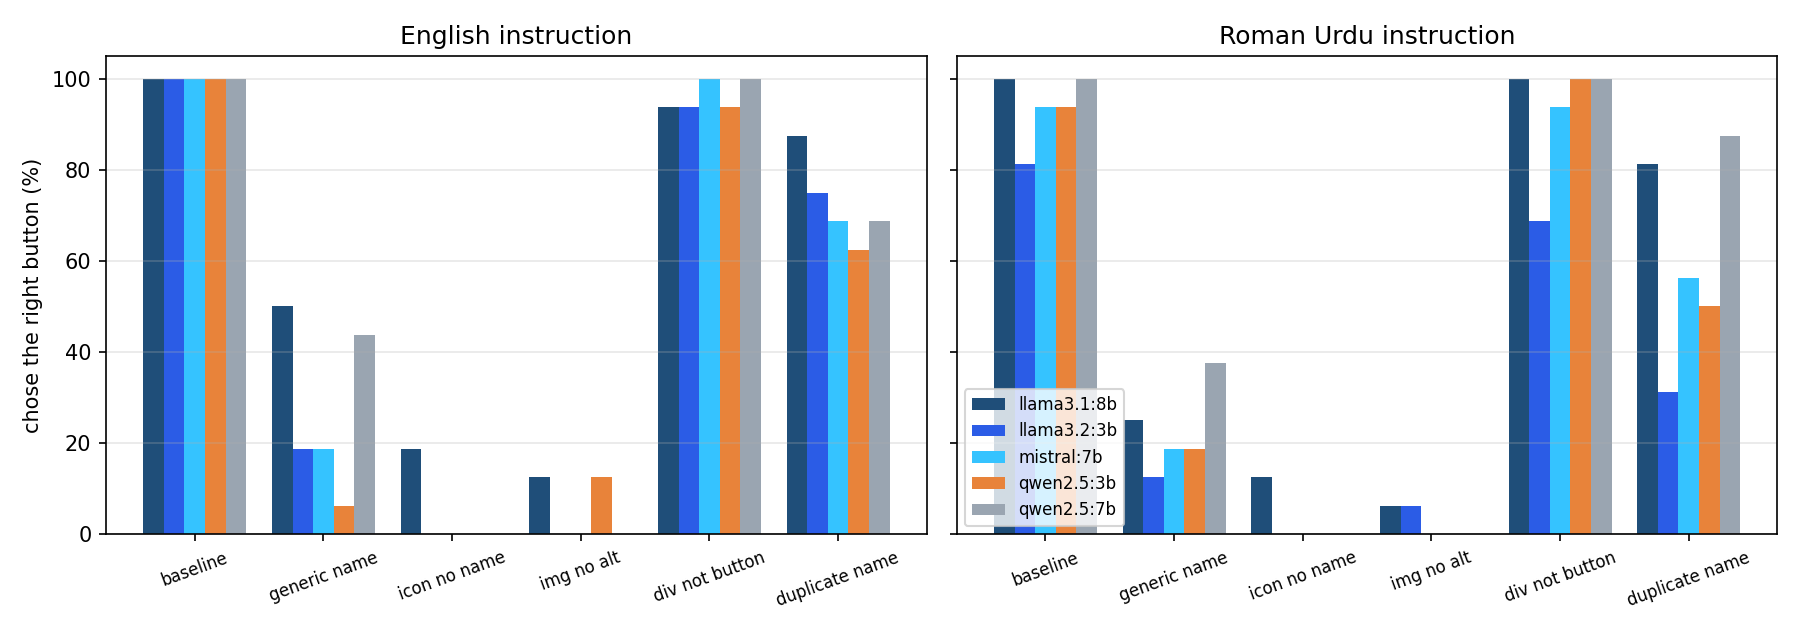
\includegraphics[width=\linewidth]{figures/fig_buttons.png}
\caption{Share of runs in which each model chose the right button, by defect, for English (left) and Roman Urdu (right) instructions; 16 runs per bar.}
\label{fig:buttons}
\end{figure}

\paragraph{How agents fail.} When the name was missing, the models did not use elimination. They chose a neutral control, a heading or the context paragraph, or replied that nothing fitted (Table~\ref{tab:pooled}). More worrying, they chose the risky look-alike in 11.9\% of runs with an unnamed icon button, 10.6\% with a generic name and 9.4\% with an image without alt text, against 1.2\% on baseline button pages. Over all button and link defects the look-alike was chosen in 62 of 1,120 runs (5.5\%), against 4 of 240 baseline runs (1.7\%). In these runs a request to save, approve or book a record would have deleted, rejected or cancelled it.

\paragraph{Models.} Every model showed the same pattern (Figure~\ref{fig:buttons}). Llama 3.1 8B was the only model to find any unnamed icon buttons (19\% English, 12\% Roman Urdu). Llama models rarely said ``none'' and so made more wrong choices (Llama 3.2 3B: 55\% of defect runs in English), while Qwen2.5 and Mistral more often abstained, which is the safer failure.

\paragraph{Roman Urdu instructions.} Over all pages, target choice in English and Roman Urdu was similar for Qwen2.5 7B (55.4\% and 56.0\%) and Llama 3.1 8B (57.7\% and 57.1\%), but lower in Roman Urdu for Llama 3.2 3B (47.0\% and 36.3\%; buttons $-14.6$ points [$-22.9$, $-7.3$]) and Mistral 7B (links $-17.5$ [$-30.0$, $-7.5$]). Even on baseline link pages, Roman Urdu instructions lowered accuracy for Qwen2.5 3B and Mistral 7B to 62\%.

\paragraph{Text fields.} A placeholder gives an input an accessible name, and four of five models found such fields as reliably as labelled ones; Qwen2.5 3B did not (25\% English). A label that is visible but not linked to the input was found in 65\% of runs, and an input with no label in 16\%.

\section{Discussion}
For these small models, the accessible name is the main signal for choosing an element. Defects that remove it, which are among the most common in practice, did not just slow the agent down; they removed its ability to act and, in about one run in ten for buttons, pointed it at a destructive neighbour. The defects that only affect the role, which break a strict script, were nearly harmless to the models because the text was still there. A developer who wants pages to work for agents should therefore fix the same names that screen-reader users need, and agent designers should treat ``no named control fits'' as a reason to stop rather than to guess.

\section{Limitations}
The pages are fictional and short, written by one person, with one defect at a time; real pages are longer and contain several defects. The task is a single element choice from the accessibility tree, not a full multi-step agent, and the models never saw the screen. We tested five small open models with default quantisation, at temperature 0 with one answer per page, and 8 to 16 pages per condition and model, so per-model intervals are wide. The look-alike is always present, which makes destructive choices possible by design. Agent behaviour is not evidence that a page works for people who use assistive technology.

\section{Conclusion}
On 168 clinic pages and 1,680 calls, five small local LLM web agents found controls with good names almost every time, found unnamed or generically named controls almost never, and sometimes chose a destructive look-alike instead. Fixing accessible names helps both people and agents.

\section*{Data and code}
Pages, code, tests, every call and the analysis: \url{https://github.com/MHKhan50/a11ybridge-accessibility-benchmark}.

\bibliographystyle{plainnat}
\bibliography{refs}
\end{document}
